\documentclass[conference]{IEEEtran}
%\IEEEoverridecommandlockouts
% The preceding line is only needed to identify funding in the first footnote. If that is unneeded, please comment it out.
\usepackage[spanish]{babel}
\usepackage[utf8]{inputenc}
\usepackage{cite}
\usepackage{amsmath, amsthm,amssymb,amsfonts}
\usepackage{algorithmic}
\usepackage{graphicx}
\usepackage{textcomp}
\usepackage{xcolor}
\def\BibTeX{{\rm B\kern-.05em{\sc i\kern-.025em b}\kern-.08em
    T\kern-.1667em\lower.7ex\hbox{E}\kern-.125emX}}

% Definición del entorno 'definition'
\newtheorem{definition}{Definición}

\begin{document}

\title{Control de Orientación de Cuerpos Rígidos\\
	% {\footnotesize \textsuperscript{*}Note: Sub-titles are not captured in Xplore and
	% should not be used}
	% \thanks{Identify applicable funding agency here. If none, delete this.}
}

\author{
	\IEEEauthorblockN{José Alejandro León Sánchez}
	\IEEEauthorblockA{\textit{Posgrado de Ingeniería} \\
		\textit{UNAM}\\
		CDMX, Mexico}
	\and
	\IEEEauthorblockN{Javier Pliego Jiménez}
	\IEEEauthorblockA{\textit{CICESE} \\
		Baja California, Mexico}
}

\maketitle

\begin{abstract}
	Este documento es un resumen de la cuarta ponencia del Seminario de Investigación de la Maestría en Ingeniería Eléctrica (Especialización en Control) del programa de Posgrado en Ingeniería de la UNAM, presentada por el Dr. Javier Pliego Jiménez. La ponencia se centró en el control de orientación de cuerpos rígidos, un problema que, a pesar de haber sido ampliamente estudiado en las últimas décadas, sigue siendo relevante debido a los desafíos teóricos y prácticos que plantea. Los sistemas involucrados son generalmente no lineales, evolucionan en espacios no euclidianos y presentan múltiples puntos de equilibrio. Se discutieron aplicaciones clave en la ingeniería aeroespacial para la orientación de satélites, así como en robótica y vehículos aéreos no tripulados (UAVs).
\end{abstract}

\begin{IEEEkeywords}
	Control de cuerpos rígidos, sistemas no lineales, satélites, robótica, UAVs
\end{IEEEkeywords}

\section{Introducción}
El control de orientación de cuerpos rígidos es un tema que ha sido objeto de investigación constante en las últimas décadas debido a su relevancia en diversos campos, como la ingeniería aeroespacial y la robótica. A nivel teórico, el problema involucra sistemas no lineales que evolucionan en espacios no euclidianos, lo que añade complejidad tanto al análisis como al diseño de controlador

Un cuerpo rígido puede definirse como un objeto tridimensional en el que la distancia entre cualquier par de puntos permanece constante a lo largo del tiempo, independientemente de las fuerzas que actúan sobre él. Para describir matemáticamente la orientación de un cuerpo rígido, es necesario utilizar un sistema de referencia que permita expresar la posición de su centro de masa (Figura 1) y sus componentes angulares. Mientras que describir la posición de un cuerpo es relativamente simple mediante un vector en un espacio euclidiano, la descripción de su orientación requiere el uso de marcos de referencia no euclidianos o transformaciones, lo que introduce desafíos adicionales en el análisis y control de estos sistemas.

\begin{figure}[h]
	\centerline{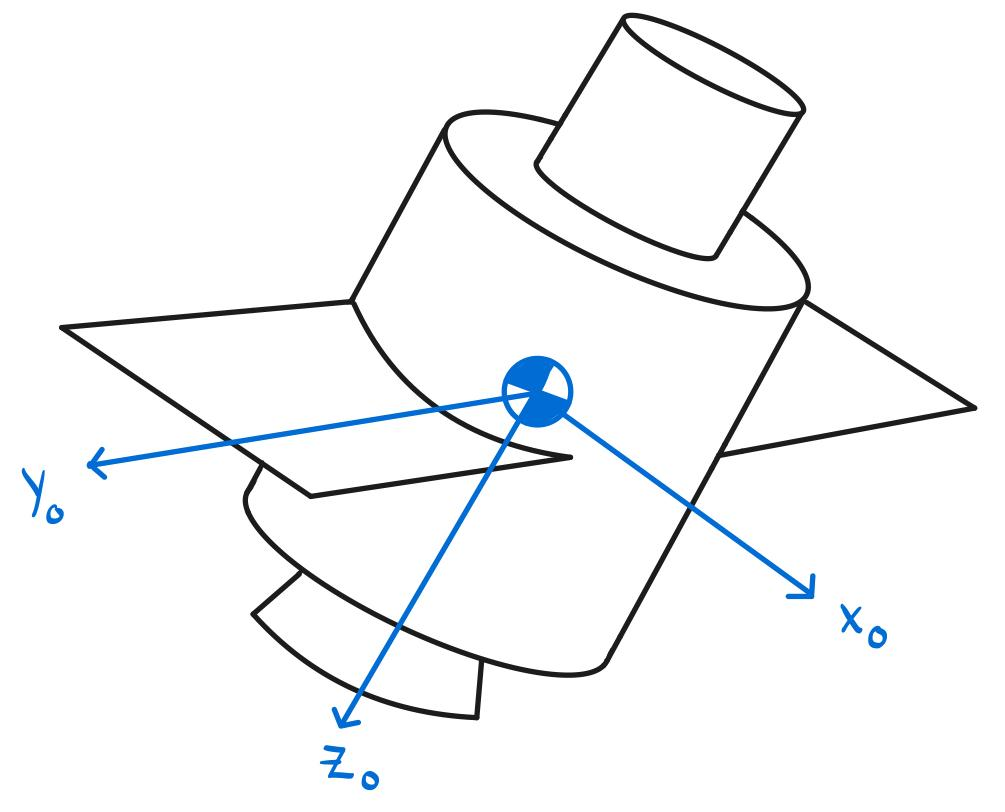
\includegraphics[width=0.3\textwidth]{satelite_cuerpo.jpeg}}
	\caption{Representación de un cuerpo rígido en un sistema de referencia.}
	\label{fig: satelite}
\end{figure}

\section{Parametrización de orientaciones}

El control de orientación de cuerpos rígidos es un problema crucial en diversas áreas de la ingeniería, como la robótica y la ingeniería aeroespacial. Para describir la orientación de un cuerpo rígido de manera matemática, es necesario introducir un sistema de referencia que permita expresar la relación entre el marco de referencia inercial y el marco del cuerpo. Este problema implica la evolución de los estados del sistema en espacios no euclidianos, particularmente en el grupo de rotaciones \( SO(3) \), lo que añade un desafío teórico y práctico en el diseño de controladores robustos.

\subsection{Ángulos de Euler}
Una de las parametrizaciones más utilizadas históricamente para representar la orientación de un cuerpo rígido es la basada en los ángulos de Euler, que consiste en una secuencia de tres rotaciones elementales alrededor de los ejes principales. La orientación del cuerpo se describe mediante tres ángulos \( (\phi, \theta, \psi) \), que corresponden a rotaciones sucesivas alrededor de los ejes de un sistema de referencia, permitiendo representar cualquier orientación posible.

A pesar de su simplicidad, los ángulos de Euler presentan limitaciones significativas, como la aparición de singularidades, lo que limita el uso global de esta parametrización.

\subsection{Cuaterniones}
Los cuaterniones, una extensión de los números complejos a \( \mathbb{R}^4 \), representan una alternativa poderosa para la descripción de rotaciones en \( SO(3) \). Un cuaternión \( q = q_0 + q_1 i + q_2 j + q_3 k \) puede describir cualquier rotación sin las singularidades inherentes a los ángulos de Euler, lo que lo convierte en una opción preferida para aplicaciones de control robusto. Esta parametrización tiene la ventaja de ofrecer una representación continua y libre de singularidades.

Sin embargo, los cuaterniones también presentan una desventaja al tener una redundancia en la representación: la orientación de un cuerpo puede describirse por dos cuaterniones opuestos \( q \) y \( -q \), lo que introduce un problema conocido como "unwinding". Este fenómeno ocurre cuando el sistema de control provoca una rotación completa innecesaria.

\subsection{Coordenadas Exponenciales}
Una tercera parametrización, basada en coordenadas exponenciales, representa una rotación en \( SO(3) \) como la exponencial de un vector \( \omega \), que describe el eje y el ángulo de rotación. Esta representación se deriva de la fórmula de Rodrigues y permite describir cualquier rotación mediante un vector de 3 dimensiones. La principal ventaja de esta parametrización radica en su capacidad para representar de manera compacta tanto las rotaciones como sus derivadas, lo que la hace especialmente útil en el diseño de controladores.

La parametrización exponencial tiene aplicaciones directas en el diseño de algoritmos de control para sistemas de orientación de cuerpos rígidos. Al evitar problemas de singularidades y "unwinding", y al ser compatible con el análisis en \( SO(3) \), es adecuada para sistemas con múltiples puntos de equilibrio y estados en espacios no euclidianos. Además, esta parametrización facilita la linealización de las ecuaciones del sistema, lo cual es clave para el diseño de controladores basados en técnicas de control no lineal.

\section{Modelos Matemáticos del Movimiento}

El comportamiento dinámico de un cuerpo rígido en un sistema de referencia móvil se puede describir utilizando un conjunto de ecuaciones diferenciales no lineales. Estas ecuaciones capturan tanto la evolución de la velocidad angular del cuerpo como el efecto del par aplicado sobre el mismo. La ecuación para la velocidad angular \( \omega \in \mathbb{R}^3 \) está dada por:

\[
	\dot{x} = J(x)\omega
\]

donde \( J(x) \in \mathbb{R}^{3x3} \) es la matriz Jacobiana que define la relación entre las velocidades generalizadas y las coordenadas del sistema. Para representar la dinámica rotacional, se utiliza la ecuación de la segunda ley de Newton para rotaciones:

\[
	M \dot{\omega} = \tau - S(\omega)M\omega
\]

Aquí, \( M \in \mathbb{R}^{3x3} \) representa la matriz de inercia, la cual es positiva definida, \( \tau \in \mathbb{R}^3 \) denota el par de fuerzas aplicadas y \( S(\omega) \) es una matriz que introduce el producto vectorial de la velocidad angular. Este conjunto de ecuaciones es fundamental para el análisis y control de cuerpos rígidos, ya que describe cómo varía la orientación del cuerpo en función del tiempo, dependiendo de las fuerzas aplicadas y las propiedades físicas del objeto.

Además, la matriz Jacobiana \( J(x) \) puede expresarse de manera explícita como:

\[
	J(x) = I_3 + \frac{1}{\|x\|^2} \left( 1 - \cos(\|x\|) \right) S^2(x) + \frac{1}{2} S(x)
\]

donde \( S(x) \) es una matriz que representa el operador de producto cruzado, permitiendo modelar las rotaciones del sistema en relación a las coordenadas del cuerpo.

\section{Algoritmos de Control}

El propósito principal en el diseño de un controlador para cuerpos rígidos es lograr que el sistema se oriente hacia una posición deseada mientras se reduce la velocidad angular a cero con el tiempo. Esto implica que la orientación \( R(t) \) debe converger a una orientación deseada \( R_d \) y la velocidad angular \( \omega \) debe tender a cero conforme \( t \to \infty \).

Para diseñar las entradas de control \( \tau \) que guíen el sistema hacia la orientación deseada, se recurre al uso de funciones de Lyapunov, las cuales permiten evaluar la estabilidad del sistema. En particular, las funciones cuadráticas o funciones barrera son comúnmente utilizadas para analizar la estabilidad, garantizando que la derivada temporal de la función de Lyapunov sea negativa definida, lo cual indica que el sistema converge hacia un equilibrio estable.

Además, al incorporar una acción integral en la ley de control, se puede asegurar estabilidad exponencial, lo que es particularmente útil en la compensación de perturbaciones constantes y acotadas que puedan estar presentes en el sistema. De esta manera, los controladores diseñados no solo estabilizan al sistema, sino que también permiten una mayor robustez frente a perturbaciones externas.


\section*{Conclusiones}

El control de la orientación de cuerpos rígidos es un problema fundamental en diversas aplicaciones, que involucra dinámicas no lineales y la evolución en espacios no euclidianos. El uso de parametrizaciones como ángulos de Euler, cuaterniones y coordenadas exponenciales, cada una con sus ventajas y limitaciones, ha permitido el desarrollo de modelos matemáticos precisos y algoritmos de control eficaces. A través de la teoría de Lyapunov, se garantiza la estabilidad del sistema y su robustez ante perturbaciones, lo que sigue siendo un área de interés para el diseño y mejora de sistemas dinámicos avanzados.

\begin{thebibliography}{00}
	\bibitem{KellySantibanez}
	R. Kelly, V. Santibañez, and A. Loría, \textit{Control of Robot Manipulators in Joint Space}. London: Springer, 2005.

	\bibitem{Spong}
	M. W. Spong, S. Hutchinson, and M. Vidyasagar, \textit{Robot Modeling and Control}. New York: John Wiley \& Sons, 2005.

	\bibitem{Solis2001}
	C. Solis, G. Barrientos, and E. Dufeu, “Alteración en el desempeño del sistema de control en manipuladores flexibles,” \textit{Mecánica Computacional}, vol. 9, pp. 367-373, 2001.

	\bibitem{SanchezPena2005}
	R. S. Sánchez-Peña and R. J. Alonso, “Control de vehículos espaciales,” \textit{Revista Iberoamericana de Automática e Informática Industrial}, vol. 2, no. 3, pp. 6-24, 2005.

\end{thebibliography}

\end{document}
